\section{Experimental Evaluation} % 70/300 points, 23%

We fine-tune and evaluate the \BertSumAbs summarization model on a A100 GPU using the Flux~\cite{InnesSFGRJKPS2018} framework on Julia~\cite{BezansonEKS2017}.
A smaller variant that we call \TransformerAbsTiny is trained on a GeForce MX150 for testing our evaluation workflow.

Describe implementation structure/approach. (Julia/Flux, data loading (\Bert, CNN, Daily Mail), tokenization (\Bert), model structure (encoder-decoder, beam search), hyperparameter tuning, optimizer)

\subsection{Dataset}

We train and evaluate the summarization model on the CNN / Daily Mail dataset~\cite{HermannKGEKSB2015}, but use preprocessed data released by \citeauthor{LiuL2019} along with the replicated paper.
From this preprocessed data we extract the source article and the target summary as raw text, join sentences to normalize separators, and tokenize with \Bert's word piece tokenizer~\cite{DevlinCLT2019}.

Describe raw data format.

Describe data preprocessing. (Pre-processed dataset from \citeauthor{LiuL2019}: Sentence splitting  with Stanford CoreNLP, entities are not anonymized.)

\subsection{Abstractive Summarizaion Model}


Describe simple tests/examples for checking implementation correctness. (Untrained model produces nonsense summaries.)

Describe implementation memory usage, complexity, and run time performance.
The full \BertSumAbs model contains 182M trainable parameters: 27M for embeddings, 85M for the encoder's transformer layers, 47M for the decoder's transformer layers, and 23M for the generator layer.

\subsection{Fine-tuning the pretrained model}

Describe training schedule.

Presumably because of the high number of parameters to tune, training this \BertSumAbs model on a A100 GPU uses about 40GB of memory at a speed of about 9 steps per minute.
Because of the slow training speed even on a powerful GPU we had to cancel training the model after 22\,500 steps.

\subsection{Beam Search}

\subsection{Experiments}

Describe experiment reproductions.

\paragraph{Training Loss}

\begin{figure}
    \centering
    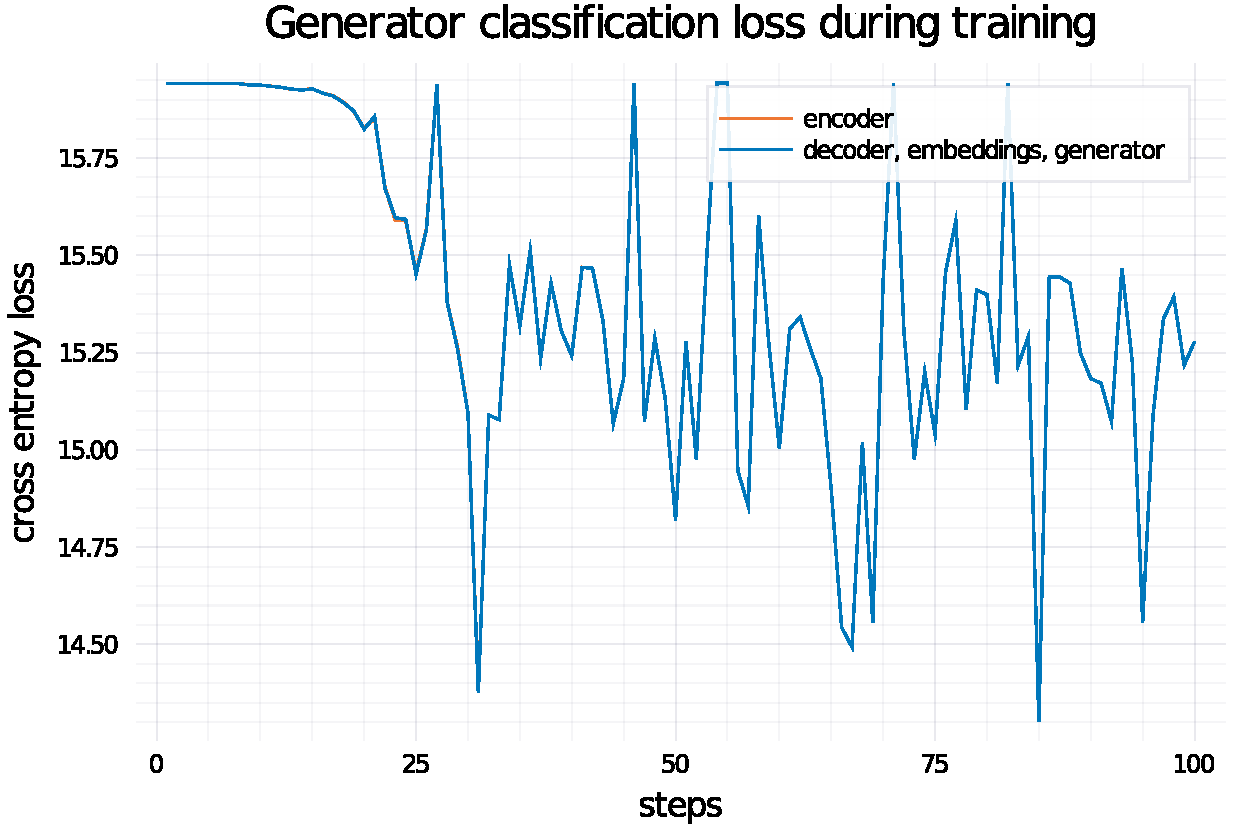
\includegraphics[width=0.7\linewidth]{training-loss-bert-abs-100.pdf}
    \caption{Cross entropy between predicted token probabilities and ground truth labels for the first 100 training steps of training the \BertSumAbs model.}
    \label{training-loss-bert-abs}
\end{figure}

\begin{figure}
    \centering
    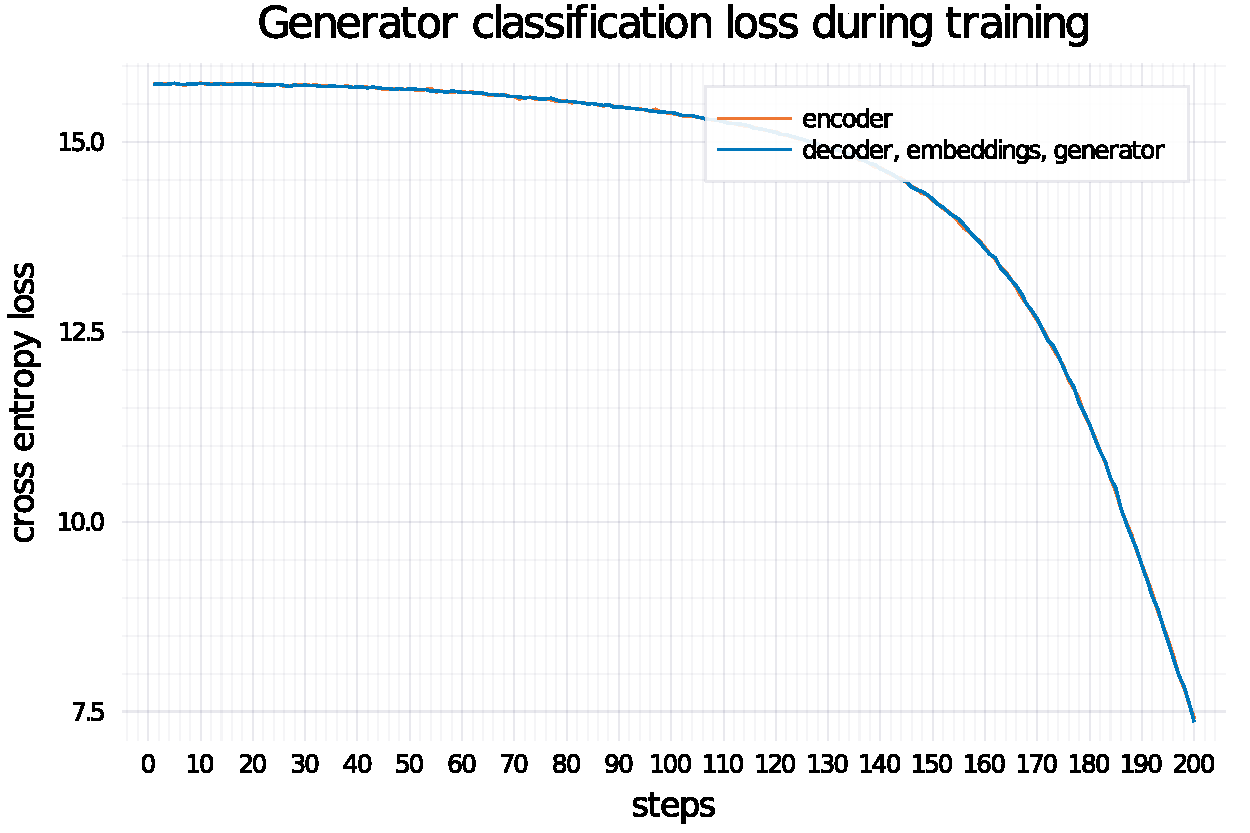
\includegraphics[width=0.7\linewidth]{training-loss-transformer-abs-tiny.pdf}
    \caption{Cross entropy between predicted token probabilities and ground truth labels for the first 200 training steps of training the \TransformerAbsTiny model.}
    \label{training-loss-transformer-abs}
\end{figure}


\paragraph{Summary Quality}

Describe \Rouge scores for some examples.

Describe/list difficulties or problems. (Pretrained data not available from a data source that allows automatic downloads.)
